%%%%%%%%%%%%%%%%%%%%%%%%%%%%%%%%%%%%%%%%%%%%%%%%%%%%%%%%%%%%%%%%%%%%
%%%%%%%%%%%%%%%%%%%%%%%%%%%%%%%%%%%%%%%%%%%%%%%%%%%%%%%%%%%%%%%%%%%%
%%                                                                %%
%% An example for writting your thesis using LaTeX                %%
%% Original version by Luis Costa,  changes by Perttu Puska       %%
%% Support for Swedish added 15092014                             %%
%%                                                                %%
%% Esimerkki opinnäytteen tekemisestä LaTeX:lla                   %%
%% Alkuperäinen versio Luis Costa,  muutokset Perttu Puska        %%
%% Ruotsinkielen tuki lisätty 05032014                            %%
%%                                                                %%
%% This example consists of the files                             %%
%% Tähän esimerkkiin kuuluu tiedostot                             %%
%%         thesistemplate.tex (versio 2.0)                        %%
%%         opinnaytepohja.tex (versio 2.0) (for text in Finnish)  %%
%%         aaltothesis.cls (versio 2.0)                           %%
%%         kuva1.eps                                              %%
%%         kuva2.eps                                              %%
%%         kuva1.pdf                                              %%
%%         kuva2.pdf                                              %%
%%                                                                %%
%%                                                                %%
%% Typeset either with                                            %%
%% Kääntäminen joko                                               %%
%% latex:                                                         %%
%%             $ latex opinnaytepohja                             %%
%%             $ latex opinnaytepohja                             %%
%%                                                                %%
%%   Result is the file opinnayte.dvi, which                      %%
%%   is converted to ps format as follows:                        %%
%%   Tuloksena on tiedosto opinnayte.dvi, joka                    %%
%%   muutetaan ps-muotoon seuraavasti                             %%
%%                                                                %%
%%             $ dvips opinnaytepohja -o                          %%
%%                                                                %%
%%   and then to pdf as follows:                                  %%
%%   ja edelleen pdf-muotoon seuraavasti                          %%
%%                                                                %%
%%             $ ps2pdf opinnaytepohja.ps                         %%
%%                                                                %%
%% Or                                                             %%
%% Tai                                                            %%
%% pdflatex:                                                      %%
%%             $ pdflatex opinnaytepohja                          %%
%%             $ pdflatex opinnaytepohja                          %%
%%                                                                %%
%%   Result is the file opinnaytepohja.pdf                        %%
%%   Tuloksena on tiedosto opinnaytepohja.pdf                     %%
%%                                                                %%
%% Explanatory comments in this example begin with                %%
%% the characters %%, and changes that the user can make          %%
%% with the character %                                           %%
%% Selittävät kommentit on tässä esimerkissä varustettu           %%
%% %%-merkeillä ja muutokset, joita käyttäjä voi tehdä,           %%
%% on varustettu %-merkeillä                                      %%
%%                                                                %%
%%%%%%%%%%%%%%%%%%%%%%%%%%%%%%%%%%%%%%%%%%%%%%%%%%%%%%%%%%%%%%%%%%%%
%%%%%%%%%%%%%%%%%%%%%%%%%%%%%%%%%%%%%%%%%%%%%%%%%%%%%%%%%%%%%%%%%%%%

%% Uncomment one of these, if you write in English:
%% the 1st when using pdflatex, which directly typesets your document in
%% pdf (use jpg or pdf figures), or
%% the 2nd when producing a ps file (use eps figures, don't use ps figures!).
\documentclass[english,12pt,a4paper,pdftex,elec,utf8]{aaltothesis}
%\documentclass[english,12pt,a4paper,dvips]{aaltothesis}

%% To the \documentclass above
%% specify your school: arts, biz, chem, elec, eng, sci
%% specify the character encoding scheme used by your editor: utf8, latin1

%%
%% Käytä toinen näistä, jos kirjoitat suomeksi:
%% ensimmäinen, jos käytät pdflatexia, joka kääntää tekstin suoraan
%% pdf-tiedostoksi (kuvat on oltava jpg- tai pdf-tiedostoina)
%% toinen, jos haluat tuottaa ps-tiedostoa (käytä eps-formaattia kuville,
%% alä käytä ps-muotoisia kuvia!)
%%
%% Use one of these if you write in Finnish:
%%
%\documentclass[finnish,12pt,a4paper,pdftex,elec,utf8]{aaltothesis}
%\documentclass[finnish,12pt,a4paper,dvips]{aaltothesis}

%% Kirjoita y.o. \documentclass optioiksi
%% korkeakoulusi näistä: arts, biz, chem, elec, eng, sci
%% editorisi käyttämä merkkikoodaustapa: utf8, latin1
%%

\usepackage{graphicx}

%% Use this if you write hard core mathematics, these are usually needed
%%
%% Matematiikan fontteja, symboleja ja muotoiluja lisää, näitä tarvitaan usein
\usepackage{amsfonts,amssymb,amsbsy}
\usepackage{epigraph}
%% Use the macros in this package to change how the hyperref package below
%% typesets its hypertext -- hyperlink colour, font, etc. See the package
%% documentation. It also defines the \url macro, so use the package when
%% not using the hyperref package.
%%
%% Jos et jostain syystä pidä, miten alla oleva hyperref-paketti käyttää
%% fontteja, värejä yms., käytä tämän paketin makroja muuttamaan
%% fonttimäärittelyt. Katso paketin dokumentaatiota. Paketti määrittelee
%% \url-makron, joten ota paketti käyttöön, jos et käytä hyperref-pakettia.
%\usepackage{url}

%% Use this if you want to get links and nice output. Works well with pdflatex.
%%
%% Saat pdf-tiedoston viittaukset ja linkit kuntoon seuraavalla paketilla.
%% Paketti toimii erityisen hyvin pdflatexin kanssa.
\usepackage{hyperref}
\hypersetup{pdfpagemode=UseNone, pdfstartview=FitH,
  colorlinks=true,urlcolor=red,linkcolor=blue,citecolor=black,
  pdftitle={Default Title, Modify},pdfauthor={Samuli Ulmanen},
  pdfkeywords={Modify keywords}}


%% All that is printed on paper starts here
%%
%% Kaikki mikä paperille tulostuu, on tämän jälkeen
\begin{document}

%% Change the school field to specify your school if the automatically
%% set name is wrong
%%
%% Korjaa vastaamaan korkeakouluasi, jos automaattisesti asetettu nimi on
%% virheellinen
% \university{aalto-yliopisto}
% \university{aalto University}
% \school{Sähkötekniikan korkeakoulu}
% \school{School of Electrical Engineering}

%% Only for B.Sc. thesis: Choose your degree programme.
%%
%% Vain kandityölle: Korjaa seuraavat vastaamaan koulutusohjelmaasi
\degreeprogram{Electronics and electrical engineering}
%\degreeprogram{Elektroniikka ja sähkötekniikka}
%%

%% ONLY FOR M.Sc. AND LICENTIATE THESIS: Specify your department,
%% professorship and professorship code.
%%
%% Vain DI/M.Sc.- ja lisensiaatintyölle: valitse laitos,
%% professuuri ja sen professuurikoodi.
\department{Department of Radio Science and Technology}
%\department{Radiotieteen ja -tekniikan laitos}

\professorship{Circuit theory}
%\professorship{Piiriteoria}
\code{S-55}
%%

%% Valitse yksi näistä kolmesta
%%
%% Choose one of these:
%\univdegree{BSc}
\univdegree{MSc}
%\univdegree{Lic}

%% Oma nimi
%%
%% Should be self explanatory...
\author{Teemu Teekkari}

%% Your thesis title comes here and again before a possible abstract in
%% Finnish or Swedish . If the title is very long and latex does an
%% unsatisfactory job of breaking the lines, you will have to force a
%% linebreak with the \\ control character.
%% Do not hyphenate titles.
%%
%% Opinnäytteen otsikko tulee tähän ja uudelleen englannin- tai
%% ruostinkielisen abstraktin yhteydessä. Älä tavuta otsikkoa ja
%% vältä liian pitkää otsikkotekstiä. Jos latex ryhmittelee otsikon
%% huonosti, voit joutua pakottamaan rivinvaihdon \\ kontrollimerkillä.
%% Muista että otsikkoja ei tavuteta!
%% Jos otsikossa on ja-sana, se ei jää rivin viimeiseksi sanaksi
%% vaan aloittaa uuden rivin.
\thesistitle{Thesis template}

\place{Espoo}

%% For B.Sc. thesis use the date when you present your thesis.
%%
%% Kandidaatintyön päivämäärä on sen esityspäivämäärä!
\date{28.2.2014}

%% B.Sc. or M.Sc. thesis supervisor
%% Note the "\" after the comma. This forces the following space to be
%% a normal interword space, not the space that starts a new sentence.
%% This is done because the fullstop isn't the end of the sentence that
%% should be followed by a slightly longer space but is to be followed
%% by a regular space.
%%
%% Kandidaattiseminaarin vastuuopettaja tai diplomityön valvoja.
%% Huomaa tittelissä "\" -merkki pisteen jälkeen,
%% ennen välilyöntiä ja seuraavaa merkkijonoa.
%% Näin tehdään, koska kyseessä ei ole lauseen loppu, jonka jälkeen tulee
%% hieman pidempi väli vaan halutaan tavallinen väli.
\supervisor{Prof.\ Pirjo Professori} %{Prof.\ Pirjo Professori}

%% B.Sc. or M.Sc. thesis advisors(s). You can give upto two advisors in
%% this template. Check with your supervisor how many official advisors
%% you can have.
%%
%% Kandidaatintyön ohjaaja(t) tai diplomityön ohjaaja(t). Ohjaajia saa
%% olla korkeintaan kaksi.
%%
%\advisor{Prof.\ Pirjo Professori}
\advisor{Lic.Sc.\ (Tech.) Janne Jalkanen}
%\advisor{M.Sc.\ Polli Pohjaaja}

%% Aalto logo: syntax:
%% Aaltologo: syntaksi:
%%
%% \uselogo{aaltoRed|aaltoBlue|aaltoYellow|aaltoGray|aaltoGrayScale}{?|!|''}
%%
%% Logo language is set to be the same as the document language.
%% Logon kieli on sama kuin dokumentin kieli
%%
\uselogo{aaltoRed}{''}

%% Create the coverpage
%%
%% Tehdään kansilehti
\makecoverpage


%% Note that when writting your master's thesis in English, place
%% the English abstract first followed by the possible Finnish abstract

%% English abstract.
%% All the information required in the abstract (your name, thesis title, etc.)
%% is used as specified above.
%% Specify keywords
%%
%% Kaikki tiivistelmässä tarvittava tieto (nimesi, työnnimi, jne.) käytetään
%% niin kuin se on yllä määritelty.
%% Avainsanat
%%
\keywords{For keywords choose concepts that are central to your thesis}
%% Abstract text
\begin{abstractpage}[english]
  Your abstract in English. Try to keep the abstract short; approximately
  100 words should be enough. The abstract explains your research topic,
  the methods you have used, and the results you obtained.
  Your abstract in English. Try to keep the abstract short; approximately
  100 words should be enough. The abstract explains your research topic,
  the methods you have used, and the results you obtained.

  Your abstract in English. Try to keep the abstract short; approximately
  100 words should be enough. The abstract explains your research topic,
  the methods you have used, and the results you obtained.
  Your abstract in English. Try to keep the abstract short; approximately
  100 words should be enough. The abstract explains your research topic,
  the methods you have used, and the results you obtained.
\end{abstractpage}

%% Force a new page so that the possible English abstract starts on a new page
%%
%% Pakotetaan uusi sivu varmuuden vuoksi, jotta
%% mahdollinen suomenkielinen ja englanninkielinen tiivistelmä
%% eivät tule vahingossakaan samalle sivulle
\newpage
%
%% Abstract in Finnish.  Delete if you don't need it.
%%
%% Suomenkielinen tiivistelmä. Poista, jos et tarvitse sitä.
%% Opinnäytteen ostikko suomeksi
\thesistitle{Opinnäyteohje}
\advisor{TkT Olli Ohjaaja}
\degreeprogram{Electronics and electrical engineering}
\department{Radiotieteen ja -tekniikan laitos}
\professorship{Piiriteoria}
%% Avainsanat
\keywords{Vastus, Resistanssi,\\ Lämpötila}
%% Tiivistelmän tekstiosa
\begin{abstractpage}[finnish]
  Tiivistelmässä on lyhyt selvitys (noin 100 sanaa)
  kirjoituksen tärkeimmästä sisällöstä: mitä ja miten on tutkittu,
  sekä mitä tuloksia on saatu.
  Tiivistelmässä on lyhyt selvitys (noin 100 sanaa)
  kirjoituksen tärkeimmästä sisällöstä: mitä ja miten on tutkittu,
  sekä mitä tuloksia on saatu.

  Tiivistelmässä on lyhyt selvitys (noin 100 sanaa)
  kirjoituksen tärkeimmästä sisällöstä: mitä ja miten on tutkittu,
  sekä mitä tuloksia on saatu.
  Tiivistelmässä on lyhyt selvitys (noin 100 sanaa)
  kirjoituksen tärkeimmästä sisällöstä: mitä ja miten on tutkittu,
  sekä mitä tuloksia on saatu.
  Tiivistelmässä on lyhyt selvitys (noin 100 sanaa)
  kirjoituksen tärkeimmästä sisällöstä: mitä ja miten on tutkittu,
  sekä mitä tuloksia on saatu.
\end{abstractpage}

%% Force new page so that the Swedish abstract starts from a new page
\newpage
%
%% Swedish abstract. Delete if you don't need it.
%%
\thesistitle{Arbetets titel}
\advisor{TkD Olli Ohjaaja} %
\degreeprogram{Electronik och electroteknik}
\department{Institutionen för radiovetenskap och -teknik}%
\professorship{Kretsteori}  %
%% Abstract keywords
\keywords{Nyckelord p\aa{} svenska,\\ Temperatur}
%% Abstract text
\begin{abstractpage}[swedish]
 Sammandrag p\aa{} svenska.
 Try to keep the abstract short, approximately
 100 words should be enough. Abstract explains your research topic,
 the methods you have used, and the results you obtained.
\end{abstractpage}

%% Preface
%%
%% Esipuhe
\mysection{Preface}
%\mysection{Esipuhe}
I want to thank Professor Pirjo Professori
and my instructor Olli Ohjaaja for their
good and poor guidance.\\

\vspace{5cm}
Otaniemi, 24.9.2016

\vspace{5mm}
{\hfill Samuli Y.\ T.\ Ulmanen \hspace{1cm}}

%% Force new page after preface
%%
%% Pakotetaan varmuuden vuoksi esipuheen jälkeinen osa
%% alkamaan uudelta sivulta
\newpage


%% Table of contents.
%%
%% Sisällysluettelo
\thesistableofcontents


%% Symbols and abbreviations
%%
%% Symbolit ja lyhenteet
\mysection{Symbols and abbreviations}
%\mysection{Symbolit ja lyhenteet}
\subsection*{Symbols}
%\subsection*{Symbolit}

\begin{tabular}{ll}
%$|a_{ij}|^2$, $|a_i|^2$ & probability of two electrons having momenta
%    $\boldsymbol p_i$ and $\boldsymbol p_j$ ($\boldsymbol p_i$ for $|a_i|^2$) \\
%                 & at any given instant \\
$\mathbf{B}$  & magneettivuon tiheys  \\
$c$              & valon nopeus tyhj\"oss\"a $\approx 3\times10^8$ [m/s]\\
%$p$              & magnitude of momentum \\
%$\boldsymbol p$, $\boldsymbol p_i$, $\boldsymbol p_i^{'}$  & momentum vector \\
%$p$              & magnitude of momentum \\
%$\boldsymbol p$, $\boldsymbol p_i$, $\boldsymbol p_i^{'}$  & momentum vector \\
%$\boldsymbol P$  &  \\
%$p_{\mathrm{F}}$ & Fermi momentum \\
$\omega_{\mathrm{D}}$    & Debye-taajuus \\
$\omega_{\mathrm{latt}}$ & hilan keskim\"a\"ar\"ainen fononitaajuus \\
$\uparrow$       & elektronin spinin suunta yl\"osp\"ain\\
$\downarrow$     & elektronin spinin suunta alasp\"ain
\end{tabular}

\subsection*{Operators}
%\subsection*{Operaattorit}

\begin{tabular}{ll}
$\nabla \times \mathbf{A}$              & vektorin $\mathbf{A}$ roottori\\
$\displaystyle\frac{\mbox{d}}{\mbox{d} t}$ & derivaatta muuttujan $t$ suhteen\\
[3mm]
$\displaystyle\frac{\partial}{\partial t}$  & osittaisderivaatta muuttujan $t$ suhteen \\[3mm]
$\sum_i $                       & Summa indeksin $i$ yli\\
$\mathbf{A} \cdot \mathbf{B}$    & vektorien $\mathbf{A}$ ja $\mathbf{B}$ pistetulo
\end{tabular}

\subsection*{Abbreviations}
%\subsection*{Lyhenteet}

\begin{tabular}{ll}
  1px & One pixel.  \\
  UA        & ''User Agent is any software that retrieves, renders and facilitates end user interaction with Web content, or whose user interface is implemented using Web technologies.''\\
URI         & ''Uniform Resource Identifiers (URIs, aka URLs) are short strings that identify resources in the web: documents, images, downloadable files, services, electronic mailboxes, and other resources. They make resources available under a variety of naming schemes and access methods such as HTTP, FTP, and Internet mail addressable in the same simple way. They reduce the tedium of "log in to this server, then issue this magic command ...'' down to a single click.''\\
\end{tabular}

%% Sivulaskurin viilausta opinn\"aytteen vaatimusten mukaan:
%% Aloitetaan sivunumerointi arabialaisilla numeroilla (ja j\"atet\"a\"an
%% leip\"atekstin ensimm\"ainen sivu tyhj\"aksi,
%% ks. alla \thispagestyle{empty}).
%% Pakotetaan lis\"aksi ensimm\"ainen varsinainen tekstisivu alkamaan
%% uudelta sivulta clearpage-komennolla.
%% clearpage on melkein samanlainen kuin newpage, mutta
%% flushaa my\"os LaTeX:n floatit
%%
%% Corrects the page numbering, there is no need to change these
\cleardoublepage
\storeinipagenumber
\pagenumbering{arabic}
\setcounter{page}{1}


%% Text body begins. Note that since the text body
%% is mostly in Finnish the majority of comments are
%% also in Finnish after this point. There is no point in explaining
%% Finnish-language specific thesis conventions in English. Someday
%% this text will possibly be translated to English.
%%
%% Leip\"ateksti alkaa
\section{Introduction}

%% Ensimm\"ainen sivu tyhj\"aksi
%%
%% Leave first page empty
\thispagestyle{empty}

Websites of today must work on a variety of screens sizes from phones, tablets to desktop. Correctly executed responsive web design allows a site to deliver an optimal user experice to an end user on any supported screen size.

Users and customers are primarily interested in quality content as contention for customers between sites is high and the decision to switch sites can be made in seconds.

The introduction of high quality screens such as the retina display on Apple platforms have put pressure to deliver high quality content on all screen sizes.

Sites usually adjust their layout according to breakpoints corresponding to well defined screen pixel widths. There may be fluid scaling between these breakpoints.

It is typical for a site to serve different scaled version of the same image for each breakpoint usually from a URI specific to each image. Images may be scaled on the UA but is generally not recommended due to varying quality on different UA's. The UA scaling is also not on par with expectations.

Serving a large sized image through a mobile network only to be scaled down later in poorer quality is a waste of the users time and the network providers' resources.

Matching image to metadata may not be done reliably by matching incoming URI to an URI to metadata mapping. In a fast paced environment it is not very valuable to the customer to add the same metadata to different versions of the same image.

For added value to the customer, reliably matching the incoming image to correct image metadata must be done on pixel data. This problem is known as Near Similar Image Matching.

Another case for using different sizes of the same image on a website is a gallery and detail view. Gallery images are smaller and provide an overview of products. The user may want or need to view a detailed view of an interesting image. Therefore two images in different scale may be needed and served from different URI's



T\"am\"an tekstin l\"ahteen\"a oleva tiedosto on opinn\"aytteen
pohja, jota voi k\"aytt\"a\"a kandidaatinty\"oss\"a, diplomity\"oss\"a ja
lisensiaatinty\"oss\"a. Tekstin
l\"ahteen\"a oleva tiedosto on kirjoitettu  \LaTeX-tiedoston rakenteen
opiskelemista ajatellen. Tiedoston kommentit sis\"alt\"av\"at
tietoa, joka on hy\"odyllist\"a opinn\"aytett\"a kirjoitettaessa.

%% Esimerkki luettelosta. Lyhyt ajatusviiva on k\"ayt\"oss\"a
%% luettelossa, ja se on pituudeltaan
%% en dash. Merkit\"a\"an latex-koodissa --.
Johdanto selvitt\"a\"a samat asiat kuin tiivistelm\"a, mutta
laveammin. Johdannossa kerrotaan yleens\"a seuraavat asiat

\begin{itemize}
\item[--]Tutkimuksen taustaa ja tutkimusaiheen yleisluonteinen esittely
\item[--]Tutkimuksen tavoitteet
\item[--]P\"a\"akysymys ja osaongelmat
\item[--]Tutkimuksen rajaus ja keskeiset k\"asitteet.
\end{itemize}

Lyhyiden opinn\"aytteiden johdannot ovat yleens\"a liian pitki\"a, joten
johdannon paisuttamista on v\"altett\"av\"a. Diplomity\"oh\"on sopii johdanto,
joka on 2--4 sivua. %% t\"ass\"a on my\"os lyhyt ajatusviiva l. en dash.
Kandidaatinty\"on johdannon on oltava diplomity\"on
johdantoa lyhyempi. Sopivasti tiivistetty johdanto ei kaipaa alaotsikoita.


%% Opinn\"aytteess\"a jokainen osa alkaa uudelta sivulta, joten \clearpage
%%
%% In a thesis, every section starts a new page, hence \clearpage
\clearpage


T\"ass\"a osassa selvitet\"a\"an, mit\"a tutkimuksen kohteena olevasta
aiheesta tiedet\"a\"an entuudestaan. Selvityksen tulee kattaa
tasapainoisesti koko tutkimuskentt\"a.

Kun opinn\"aytety\"ot\"a kirjoitetaan, on noudatettava
ohjeita, jotka koskevat opinn\"aytteen rakennetta,
k\"ayt\"ant\"oj\"a, muotoseikkoja sek\"a ulkoasua. Esitell\"a\"an n\"ait\"a
ohjeita tarkemmin.

%% Osan hienojaottelua alaosiin, eik\"a v\"altt\"am\"att\"a edes tarpeen,
%% t\"ass\"a vain esimerkkin\"a. K\"ayt\"a harkintasi mukaan
%% osan jaottelua, joskus alaotsikot selvent\"av\"at asioita ja
%% joskus vain sirpaloittavat tarpeettomasti teksti\"a.
%%  Jaottelu menee seuraavasti:
%% \section{osan otsikko}
%% \subsection{alaotsikko}
%% \subsubsection{ala-alaotsikko}
%% T\"at\"a pitem\"alle ei pid\"a jaotella.
%%
%% Three levels of hierarchy in sectioning should be enough

\subsection*{Rakenne}

Opinn\"aytteen rakenteen tulee olla hyv\"an tieteellisen
kirjoittamisen k\"ayt\"ann\"on mukainen ja sis\"alt\"a\"a v\"ahint\"a\"an seuraavat
osat:

\begin{enumerate}
\item Nimi\"olehti
\item Tiivistelm\"a
\item Sis\"allysluettelo
\item Symboli- ja lyhenneluettelo
\item \label{a} Johdanto
%% T\"ass\"a alla on esimerkki lainausmerkkien k\"ayt\"ost\"a. Suomalaisen tekstin
%% lainausmerkit eiv\"at mene oikein latexissa (tai monissa muissakaan
%% julkaisuj\"arjestelmiss\"a) kun k\"aytet\"a\"an
%% "-merkki\"a, koska latex k\"aytt\"a\"a amerikkalaista lainausmerkkien
%% tulostustapaa. Vaihtoehtona voi k\"aytt\"a\"a kulmalainausmerkkej\"a, jotka
%% my\"os tulostuvat oikein.
\item  Aikaisempi tutkimus. Ty\"on luonteen niin vaatiessa otsikko voi olla my\"os
        >>Teoreettinen tausta>>  tai n\"aiden otsikoiden yhdistelm\"a.
\item Tutkimusaineisto ja -menetelm\"at %% yhdysmerkki - eli tavuviiva.
\item Tulokset
\item \label{o} Tarkastelu. Ty\"on luonteen niin vaatiessa otsikko voi
      olla my\"os >>Johtop\"a\"at\"okset>> tai >>Yhteenveto>>
      tai edell\"a mainittujen otsikoiden yhdistelm\"a.
\item L\"ahteet
\item Liitteet.
\end{enumerate}

Tiivistelm\"an ja symboli- sek\"a lyhenneluetteloiden
v\"aliin voi sijoittaa halutessaan esipuheen.

Ty\"on osat \ref{a}-\ref{o} muodostavat \textit{tekstiosan.}  Ty\"on
yksitt\"aisi\"a osia voidaan jakaa alaotsikoilla alaosiin, joita ei ole
yll\"a esitetty. Alaotsikoiden k\"aytt\"aminen selvent\"a\"a parhaimmillaan
teksti\"a, ja pahimmillaan sirpaloittaa sit\"a.  Sirpaloitumista voi est\"a\"a
huolehtimalla siit\"a, ett\"a samalla sivulla ei esiinny useampaa
alaotsikkoa.  Tekstin j\"asentelyss\"a on yleens\"a ongelmia, jos osassa on
vain yksi alaosa, tai kirjoittaja joutuu k\"aytt\"am\"a\"an useampaa kuin
kahta tasoa (osa ja alaosat): alaosien alaosat ovat harvoin tarpeen.
\subsection*{Sivut ja kirjaintyypit}

Opinn\"aytteen tulee olla kirjoitettu koneella tai
tekstink\"asittelyohjelmalla yksipuolisesti A4-kokoiselle paperille.
Kandidaatinty\"on tekstiosan sopiva pituus on noin 15--20 sivua ja
diplomity\"on noin 60 sivua. Ty\"ot\"a ei ole syyt\"a tarpeettomasti pident\"a\"a.

Opinn\"aytteen tekstiosan kirjaintyypin tulee olla antiikva eli
%% esimerkki pakkotavutuksesta; "serif-tyyppinen" on tavutuksen kannalta
%% hankala, joten pakkotavutetaan se.
serif\--tyyp\-pi\-nen ja lis\"aksi kursivoimaton, lihavoimaton sek\"a kooltaan 12
pistett\"a (kuten t\"ass\"a esityksess\"a). Groteskeja eli \textsf{Sans
  serif}-tyyppisi\"a kirjaintyyppej\"a (kuten Helvetica tai Arial) ei saa
k\"aytt\"a\"a varsinaisessa tekstiss\"a, mutta otsikoissa n\"ait\"a voidaan
k\"aytt\"a\"a.  Otsikoissa voidaan k\"aytt\"a\"a kooltaan edell\"a mainittua
suurempaa kirjaintyyppi\"a sek\"a tyylikeinoja, kuten lihavointia tai
kursivointia.  Tekstiss\"a samantasoisten otsikoiden on kuitenkin oltava
tyylilt\"a\"an ja kirjainlajeiltaan yhtenev\"aisi\"a.
%% Esimerkki taulukosta
\begin{table}[htb]
%% Taulukon teksti
\caption{Taulukoissa ja kuvissa kirjaintyypin voi valita
tarkoituksenmukaisesti, mutta kuva- ja taulukkoteksteiss\"a tulee
k\"aytt\"a\"a samaa kirjaintyyppi\"a kuin varsinaisessa tekstiss\"a.
Huomaa taulukon numeroinnin sijoittuminen taulukon yl\"apuolelle. \label{taulukko1}}
\begin{center}
\fbox{
\begin{tabular}{c|l|r}
\textbf{A} & 1 & $e^{j \omega t}$ \\ \hline
\textsf{B} & 2 & ${\mathfrak R}(c)$ \\ \hline
\texttt{C} & 3 & $ a \in \mathbb{A}$
\end{tabular}
}
\end{center}
\end{table}

Opinn\"aytteen vasen marginaali (sidonnan puoli) on
35~mm % t\"ass\"a ~ muodostaa ns. yhdist\"av\"an v\"alily\"onnin
ja oikea 25~mm. Yl\"amarginaali on 25~mm. Leip\"atekstin korkeus on
enimmill\"a\"an 230mm. T\"am\"an opinn\"aytepohjan marginaalien pit\"aisi olla
paperille tulostettuna oikein, mutta tulostimesta ja paperista
riippuen voi esiinty\"a yhden tai kahden millimetrin suuruisia eroja.
%% Jos k\"a\"ann\"at t\"am\"an tekstin pdflatex-komennolla ja tulostat sen katselu-
%% ohjelmasta, toteat todenn\"ak\"oisesti em. mittojen poikkeavan enemm\"an
%% kuin 1-2 mm.
%% T\"am\"a on seurausta pdf-tiedoston erilaisesta kirjaintyyppim\"a\"arityksest\"a.
%% Korkeatasoista painoty\"ot\"a varten k\"ayt\"a vain latex-komentoa ja
%% tulosta postscript-muotoon k\"a\"annetyst\"a tiedostosta.
\subsection*{Asemointi}

%% Muutos vanhaan ohjeeseen verrattuna: aikaisemmassa ohjeessa
%% kehotettiin k\"aytt\"am\"a\"an vasensuora-asettelua, mutta t\"ass\"a
%% ohjeessa ollaan luovuttu tuosta vaatimuksesta ja siirrytty
%% huoliteltumpaan, painotuotteenomaisempaan suuntaan.
Tekstiosan tekstiss\"a k\"aytet\"a\"an kappaleiden erottamiseen sisennyst\"a,
mutta ensimm\"aist\"a otsikon, v\"aliotsikon tai muun katkon j\"alkeist\"a
kappaletta ei sisennet\"a. Jos kuva tai muu katko tulee kappaleiden
v\"aliin, suositellaan katkon j\"alkeisen kappaleen sisent\"amist\"a.

Mik\"ali oikea reuna halutaan tasata, tulee k\"aytt\"a\"a tavutusta ja lis\"aksi
tarkistaa, ettei tekstiin j\"a\"a lukemista h\"airitsevi\"a pitki\"a sanav\"alej\"a. Jos
k\"ayt\"at opinn\"aytteen tekemisess\"a \LaTeX-j\"arjestelm\"a\"a,
t\"am\"a asia hoituu automaattisest.

Opinn\"aytteen riviv\"ali on 1, mik\"a on my\"os t\"am\"an opinn\"aytepohjan k\"ayt\"ant\"o.
Kappaleiden tulee yleens\"a olla ainakin kolmen rivin pituisia, mutta
my\"os liian pitki\"a kappaleita tulee v\"altt\"a\"a.  T\"ass\"a opinn\"aytepohjassa
ei tekstin luonteen vuoksi voida t\"aysin toteuttaa kappaleen pituutta koskevia
vaatimuksia.

Yksitt\"aisi\"a, kappaleen p\"a\"att\"avi\"a tai aloittavia rivej\"a sivun alussa
tai lopussa on v\"altett\"av\"a koko ty\"oss\"a, my\"os luetteloissa ja
liitteiss\"a.

\subsection*{Numerointi}

Opinn\"aytteen jokainen osa alkaa uudelta sivulta. Alaosa aloittaa uuden
sivun vain edellisen sivun t\"aytytty\"a.

Ty\"on osat numeroidaan siten, ett\"a johdanto on ensimm\"ainen numeroitava
osa. Osien numeroinnissa k\"aytet\"a\"an arabialaisia numeroita.

Nimi\"olehti, tiivistelm\"a, esipuhe, sis\"allysluettelo ja symboli- ja
lyhenneluettelo numeroidaan esipuheesta tai t\"am\"an puuttuessa
ensimm\"aiselt\"a luettelosivulta alkaen roomalaisin numeroin.

Sivunumerointi alkaa toiselta varsinaiselta tekstisivulta, ja
sivunumeroinnissa k\"aytet\"a\"an arabialaisia numeroita.

L\"ahdeluettelo alkaa uudelta sivulta. L\"ahdeluettelon sivunumerointi
jatkuu viimeisest\"a tekstisivusta.

Jokainen liite alkaa uudelta sivulta. Liitteiden sivunumerointi
jatkuu viimeisest\"a l\"ahdeluettelon sivusta.

Sivunumero sijoitetaan sivun yl\"areunaan.

Matemaattiset kaavat numeroidaan arabialaisin
numeroin. Kaavanumerointi ei saa katketa osien v\"aliss\"a (eik\"a niin
tapahdukaan, jos k\"ayt\"at t\"at\"a opinn\"aytepohjaa). Kaikkia kaavoja ei tarvitse
numeroida, vaan kirjoittaja voi k\"aytt\"a\"a harkintaa numeroinnin
tarpeellisuudessa.  Liitteiss\"a olevat kaavat numeroidaan siten, ett\"a
liitteen ajatellaan muodostavan numeroinnin kannalta itsen\"aisen ja
yhten\"aisen kokonaisuuden. Kaavan numero sijoitetaan oikealle puolelle
alla olevan esimerkin mukaisesti
\begin{equation}
D(xy) = (Dx)y + x(Dy),  \hspace{3em} x,y \in \mathbb{A}.
\end{equation}
%% Kaavojen j\"alkeen ei yleens\"a laiteta sisennyst\"a.
Kaikki kuvat ja taulukot numeroidaan erillisen juoksevan numeroinnin
mukaisesti kuten taulukosta \ref{taulukko1} ja kuvasta \ref{kuva1} k\"ay
ilmi.  Liitteiss\"a olevat kuvat ja taulukot numeroidaan siten, ett\"a
liitteen ajatellaan muodostavan numeroinnin kannalta itsen\"aisen ja
yhten\"aisen kokonaisuuden. Liitteiss\"a \ref{LiiteA} ja \ref{LiiteB} on
esimerkkej\"a kaavojen (kaavat \ref{liitekaava1}--\ref{liitekaava2} tai
kaavat \ref{liitekaava3}--\ref{liitekaava4}), kuvien (kuva
\ref{liitekuva}) ja taulukoiden (taulukko \ref{liitetaulukko})
numeroimisesta.  Liitteet numeroidaan suuraakkosin (esimerkiksi Liite
A, Liite B tai pelk\"ast\"a\"an A, B).
%% T\"ass\"a esimerkki kuva1.pdf -nimisen tiedoston tuomisesta kuvaksi.
%% Komento \inclugraphics[parametrit]{argumentti} tuo kuvan.
%% Komento \centering pakottaa kuvan keskelle.
%% Komento \caption luo kuvatekstin ja sen numeroinnin
%% Parametrit htb pakottavat kuvan suunnilleen siihen
%% kohtaan, miss\"a se esiintyy tekstin l\"ahdekoodissa
\begin{figure}[htb]
\centering 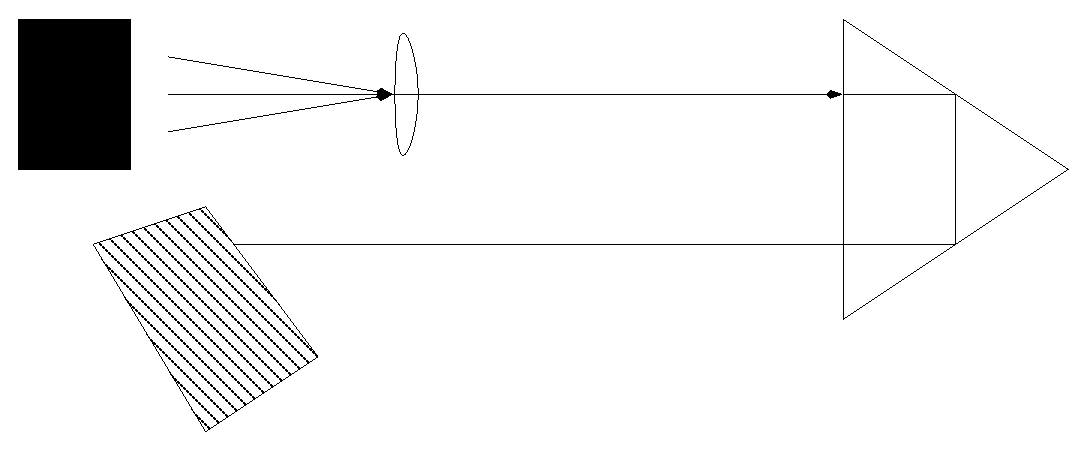
\includegraphics[height=5cm]{kuva1}
\caption{T\"am\"a on esimerkki numeroidusta kuvatekstist\"a. \label{kuva1}}
\end{figure}

\subsection*{L\"ahdeviittausten k\"aytt\"o}

L\"ahdeviittaukset tulee tehd\"a huolellisesti ja johdonmukaisesti
numeroviitej\"arjestelm\"an mukaisesti. Numeroviitteet j\"arjestet\"a\"an
l\"ahdeluetteloon viittausj\"arjestykseen, mutta jos l\"ahdeluettelo
on hyvin laaja (useita sivuja), j\"arjestet\"a\"an viitteet p\"a\"asanan
mukaiseen aakkosj\"arjestykseen. Alaviitej\"arjestelm\"a\"a
\footnote{My\"osk\"a\"an alaviitteen\"a olevia kommentteja \underline{ei} suositella
k\"aytett\"aviksi.} ei k\"aytet\"a.

Viitteen sijoittelussa noudatetaan seuraavia s\"a\"ant\"oj\"a:
Jos viite kohdistuu vain yhteen virkkeeseen tai virkkeen
osaan, viite \cite{Kauranen} sijoitetaan virkkeen sis\"a\"an ennen virkett\"a
p\"a\"att\"av\"a\"a pistett\"a. Jos taas viite koskee tekstin useampaa
virkett\"a tai kokonaista kappaletta, sijoitetaan viite kappaleen loppuun
pisteen j\"alkeen. \cite{Kauranen}

\subsection*{L\"ahdeluettelo}

L\"ahdeluettelossa esiintyy tavallisesti seuraavassa esitett\"avi\"a
l\"ahteit\"a, joista on numeroviitej\"arjestelm\"ass\"a ilmoitettava
asianomaisessa kohdassa vaaditut tiedot.

%% Esimerkki korostamisesta. Lihavoinnin sijasta on tyylikk\"a\"amp\"a\"a
%% ja luettavampaa k\"aytt\"a\"a kursiivia.
\textit{Kirjasta} ilmoitetaan seuraavat tiedot:

\begin{itemize}
\item[--]tekij\"at
\item[--]julkaisun nimi
\item[--]painos, jos useita
\item[--]kustannuspaikka
\item[--]julkaisija tai kustantaja
\item[--]julkaisuaika
\item[--]mahdollinen sarjamerkint\"o.
\end{itemize}

Viitteet \cite{Kauranen}--\cite{Koblitz} ovat esimerkkej\"a kirjan
esitt\"amisest\"a l\"ahdeluettelossa. Viite \cite[s.\ 83--124]{Koblitz} on
esimerkki l\"ahdeluettelossa esiintyv\"an kirjan tiettyjen sivujen
esitt\"amisest\"a tekstiss\"a.

\textit{Artikkelista} kausijulkaisussa ilmoitetaan seuraavat tiedot:

\begin{itemize}

\item[--]tekij\"at
\item[--]artikkelin nimi
\item[--]kausijulkaisun nimi
\item[--]julkaisuvuosi
\item[--]kausijulkaisun volyymi tai ilmestymisvuosi
\item[--]kausijulkaisun numero
\item[--]sivut, joilla artikkeli on.
\end{itemize}

Viitteet \cite{bcs}--\cite{Deschamps} ovat esimerkkej\"a artikkelin
esitt\"amisest\"a l\"ahdeluettelossa.

\textit{Kokoomateoksen luvusta tai osasta} ilmoitetaan seuraavat tiedot:

\begin{itemize}
\item[--]luvun tai osan tekij\"at
\item[--]luvun tai osan nimi
\item[--]maininta >>Teoksessa>>
\item[--]koko teoksen toimittajat sek\"a maininta >>(toim.)>>
\item[--]koko teoksen tai konferenssin nimi
\item[--]konferenssiesitelm\"an kyseess\"a ollessa sen pitopaikka ja -aika
\item[--]painos, jos useita
\item[--]kustannuspaikka
\item[--]julkaisija tai kustantaja, jos aihetta t\"am\"an ilmoittamiseen on
\item[--]julkaisuaika
\item[--]sivut, joilla luku tai osa on
\item[--]mahdollinen sarjamerkint\"a.
\end{itemize}

Viitteet \cite{Sihvola}--\cite{Lindblom} ovat esimerkkej\"a
kokoomateoksen luvun tai osan esitt\"amisest\"a l\"ahdeluettelossa.

\textit{Opinn\"aytety\"ost\"a} ilmoitetaan seuraavat tiedot:

\begin{itemize}
\item[--]tekij\"a
\item[--]ty\"on nimi
\item[--]opinn\"aytety\"on tyyppi
\item[--]oppilaitoksen nimi
\item[--]osaston, laitoksen tai ohjelman nimi
\item[--]oppilaitoksen sijaintipaikka
\item[--]vuosiluku.
\end{itemize}

Viitteet \cite{Miinusmaa}--\cite{Lonnqvist} ovat esimerkkej\"a
opinn\"aytteen esitt\"amisest\"a l\"ahdeluettelossa.

\textit{Standardista} ilmoitetaan seuraavat tiedot:

\begin{itemize}
\item[--]standardin tunnus ja numero
\item[--]standardin nimi
\item[--]painos, mik\"ali ei ole ensimm\"ainen
\item[--]julkaisupaikka
\item[--]julkaisija
\item[--]julkaisuvuosi
\item[--]sivum\"a\"ar\"a.
\end{itemize}
Viite \cite{sfs} on esimerkki standardin esitt\"amisest\"a opinn\"aytteen
l\"ahdeluettelossa.

\textit{Haastattelusta} ilmoitetaan seuraavat tiedot:

\begin{itemize}
\item[--]haastatellun henkil\"on nimi
\item[--]haastatellun henkil\"on arvo tai asema
\item[--]haastatellun henkil\"on edustama organisaatio
\item[--]organisaation osoite
\item[--]maininta siit\"a, ett\"a kyseess\"a on haastattelu ja haastattelun
p\"aiv\"am\"a\"ar\"a.
\end{itemize}

Viite \cite{haastattelu} on esimerkki
haastattelun esitt\"amisest\"a l\"ahdeluettelossa.

Osa s\"ahk\"oisess\"a muodossa olevista artikkeleista on saatavissa my\"os
painettuina. \textit{Vain verkosta saatavissa olevasta artikkelista} esitet\"a\"an
seuraavat tiedot:

\begin{itemize}
\item[--]tekij\"at
\item[--]artikkelin nimi
\item[--]kausijulkaisun nimi
\item[--]viestintyyppi
\item[--]laitos tai volyymi
\item[--]kausijulkaisun yksitt\"aist\"a osaa koskeva merkint\"a tai numero
\item[--]julkaisuvuosi tai maininta >>P\"aivitetty>> ja p\"aivitysaika
\item[--]maininta >>Viitattu>> ja viittaamisen ajankohta
\item[--]maininta >>Saatavissa>> ja URL tai
\item[--]maininta >>DOI>> ja DOI-numero (DOI=Digital Object Identifier).
\end{itemize}

Viitteet \cite{Ribeiro}--\cite{kone} ovat esimerkkej\"a s\"ahk\"oisess\"a
muodossa olevan artikkelin esitt\"amisest\"a opinn\"aytteen
l\"ahdeluettelossa.  Viitteet \cite{Ribeiro} ja \cite{Stieber} ovat
saatavissa sek\"a painettuna ett\"a verkosta, joten viitteiden esitystapa
mukailee painetun artikkelin viitteen esitystapaa, mutta sen lis\"aksi
kerrotaan julkaisun olevan verkkolehti ja lehden olevan saatavissa
my\"os painettuna.  Viite \cite{kone} on saatavissa vain verkosta ja
siit\"a esitet\"a\"an yll\"a vaaditut tiedot.

Valitettavasti s\"ahk\"oisess\"a muodosssa olevasta artikkelista ei ole aina
saatavissa lai\-tos-, volyymi- tai numerotietoja.

\textit{S\"ahk\"oisess\"a muodossa olevasta opinn\"aytety\"ost\"a} ilmoitetaan
seuraavat tiedot:

\begin{itemize}
\item[--]tekij\"a
\item[--]ty\"on nimi
\item[--]viestintyyppi
\item[--]opinn\"aytety\"on tyyppi
\item[--]oppilaitoksen nimi
\item[--]osaston, laitoksen tai ohjelman nimi
\item[--]oppilaitoksen sijaintipaikka
\item[--]vuosiluku
\item[--]viittamisen ajankohta
\item[--]maininta >>Saatavissa>> ja URL tai
        maininta >>DOI>> ja DOI-numero.
\end{itemize}

Viite \cite{Adida} on esimerkki s\"ahk\"oisess\"a muodossa olevan
opinn\"aytteen esitt\"amisest\"a l\"ahdeluettelossa.

Viite \cite{viittaaminen} on esimerkki itsen\"aisen kirjoituksen sis\"alt\"av\"ast\"a
verkkosivusta. T\"allainen l\"ahde on rinnastettavissa erillisteokseen.
\textit{Verkkosivusta} esitet\"a\"an tiedot:

\begin{itemize}
\item[--] tekij\"at
\item[--] otsikko
\item[--] maininta >>P\"aivitetty>> ja p\"aivitysaika
\item[--] maininta >>Viitattu>> ja viittaamisen ajankohta
\item[--] Maininta >>Saatavissa>> ja URL.
\end{itemize}

Joskus verkkosivun kirjoitus on jaettu useammalle sivulle, jolloin
l\"ahdeluetteloon kirjataan vain sellainen verkko-osoite, joka koskee
koko kirjoitusta tai sen etusivua, ellei sitten
todella tarkoiteta kirjoituksen yksitt\"aist\"a sivua.

\subsection*{Muuta huomioitavaa l\"ahdeluettelossa}

%% Muutos vanhoihin ohjeisiin koskien kielt\"a.
L\"ahdeluettelossa ty\"on ja julkaisun nimi kirjoitetaan alkuper\"aisess\"a
muodossaan. Julkaisijan kotipaikka kirjoitetaan alkukielisess\"a
muodossaan.

Viittamista koskevassa suomalaisessa standardissa
SFS 5342 \cite{sfs} vaaditaan julkaisuista ilmoitettavaksi my\"os ISBN- tai
ISSN-numerot, mutta n\"aiss\"a opinn\"ayteohjeissa ei ISBN- ja
ISSN-numeroita vaadita.

\clearpage

\section{Materials and methods}

\subsection{Evaluating classifiers}
To compare the dct-, and simple perceptual hash classifiers to large scale image retrieval by SIFT features in a systematic way, we will use receiver operating characteristic \(ROC\) graphs to visualize the performance of each classifier and compare their performance.

In our case the image is classified correctly by the classification system or it is not. This is a binary classification problem. The confusion matrix can be found in figure \ref{figconfusion}.

\begin{figure}[htb]
\begin{center}
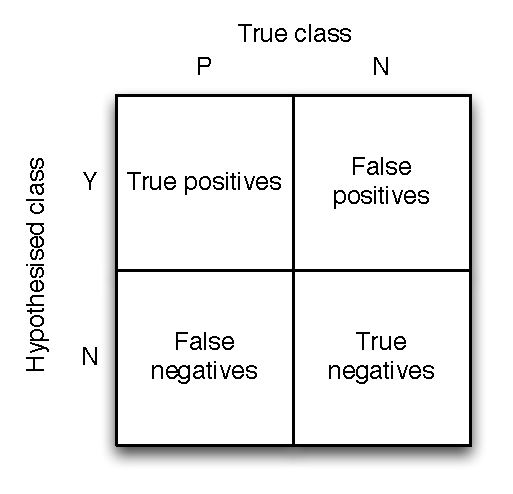
\includegraphics[height=8cm]{figures/confusion}
\end{center}
\caption{Confusion matrix for binary classification \cite{Fawcett2006}. }
\label{figconfusion}
\end{figure}



\subsection{Near duplicate images}
Definitions can vary depending on the problem at hand from finding exact matches to matching images with the same scene or object.

Our requirements for a classifier are high true positive rate, a high true negative rate, and a low false positive rate. of an image at different scales. Customer is reporting 20\% to 30\% misses (false negatives) for dct hash and reporting that the simple hash is also missing too many images. We are going to keep the problem the same, but attempt to widen the definition to the same scene or object and in this way to reduce misses while keeping the false positive rate extremely low.

\subsection{Perceptual hashing}
Near similar image detection is done via perceptual hashing due to their simplicity. They are simple to implement and inexpensive to compute. Hashes are not calculated for if image widht or height is less than 32px. Adding metadata to an image that small is counterproductive.


\subsubsection{Simple hash}

\subsubsection{DCT Hash}

\begin{equation}
X_{k_1,k_2} = \sum_{n_1=0}^{N_1-1} \sum_{n_2=0}^{N_2-1}x_{n_1,n_2}cos\left[\frac{\pi}{N_1}\left(n_1+\frac{1}{2}\right)k_1\right]cos\left[\frac{\pi}{N_2}\left(n_2+\frac{1}{2}\right)k_2\right]
\end{equation}

\subsection{Large scale image retrieval by SIFT features}

\subsection{Simulation}
\epigraph{Without data you're just another person with an opinion}{W. Edwards Deming}

To compare object instance recognition by SIFT features to perceptual hashing we will run simulations on matlab. We are faced with a binary classification problem. Receiver operating characteristics have been useful for visualizing classifier performance \cite{Fawcett2006}. We will construct ROC graphs for the simple hash, dct hash and large scale image retrieval with SIFT features.

To begin production implementation solving the near similar image matching problem with SIFT-features we need to know if the new solution is an improvement over the existing what we call the simple hash and a version DCT hash. A set of images is needed, as well as well as a modified set described in table \ref{modifiedimages} simulating scenarios typically encountered in duplicate image detection.

\def\arraystretch{1.5}
\begin{table}[htb]
\caption{Test image sets and motivations taken from the "Recognition of object instances practical" paintings set of images.}
\label{modifiedimages}
\begin{center}
\begin{tabular}{lp{0.5\linewidth}}
  Modification & Motivation \\
  \hline \hline
  53\% scale& Simulate responsive site case where image has a scaled duplicate. Choose prime percentage to avoid multiple of two to push scaler to produce uneven results.\\
  \hline
  83\% scale& Another scaled case \\
  \hline
  Shave 10px & Simulate cropping image by 10px or removing a border for example\\
  \hline
  Shave 20px & Simulate cropping image by 20px or removing a border for example\\
  \hline
  10\% border & Adding a border to a known image \\
  \hline
  Rotate 10\% & User corrects the horizon of a photo \\
  \hline
  Normalize histogram & User normalizes the histogram of a photo\\
  \hline
  Saturate colors & User decides to modify the color palette of the image or photo\\
  \hline
  Horizontal flip & User uses a mirror image. Pushing near duplicate detection to the limit\\
  \hline
  Vertical flip & User flips the image vertically. We push near duplicate detection to the limit\\
  \hline
\end{tabular}
\end{center}\end{table}


Paintings dataset from the "Recognition of object instances practical" http://www.robots.ox.ac.uk/~vgg/practicals/instance-recognition/index.html of a total of 1708 images will be used due to ready scripts for the SIFT case.

A shell script using imagemagick will create manipulated duplicates. 53\% and 83\% scales. In addition a case were the image horizon is fixed by a slight rotation is a usual case so we will use a 10\% rotation. Increased saturation is chosen for color manipulation so we will saturate the image by 50\%. Histogram normalization is quite a common operation, so we will use a normalized version of the image to try to find matches.

To simulate cropped images we will use 10\% and 20\% cropping. Adding a border is also a common operation so that case is simulated by making duplicates with a 10px border.

In order to test for images not in the set we will pick 1708 images from the ThingLink database and run those images against the set. This will look for a false positive rate with images that are not in the dataset at all.

\clearpage

\section{Results}

T\"ass\"a osassa esitet\"a\"an tulokset ja vastataan tutkielman alussa
esitettyihin tutkimuskysymyksiin. Tieteellisen kirjoitelman
arvo mitataan t\"ass\"a osassa esitettyjen tulosten perusteella.

%% Huomaa seuraavassa kappaleessa lainausmerkkien ulkopuolella piste,
%% koska piste ei lopeta lainattua tekstinp\"atk\"a\"a.
%% Jos lainattu tekstinp\"atk\"a loppuu v\"alimerkkiin, tulee v\"alimerkki
%% lainausmerkkien sis\"alle:
%% "Et tu, Brute?" sanoi Caesar kuollessaan.
Tutkimustuloksien merkityst\"a on aina syyt\"a arvioida ja tarkastella
kriittisesti.  Joskus tarkastelu voi olla t\"ass\"a osassa, mutta se
voidaan my\"os j\"att\"a\"a viimeiseen osaan, jolloin viimeisen osan nimeksi
tulee >>Tarkastelu>>. Tutkimustulosten merkityst\"a voi arvioida my\"os
>>Johtop\"a\"at\"okset>>-otsikon alla viimeisess\"a osassa.

T\"ass\"a osassa on syyt\"a my\"os arvioida tutkimustulosten luotettavuutta.
Jos tutkimustulosten merkityst\"a arvioidaan >>Tarkastelu>>-osassa,
voi luotettavuuden arviointi olla my\"os siell\"a.

\clearpage

\section{Discussion}

Opinn\"aytteen tekij\"a vastaa siit\"a, ett\"a opinn\"ayte on t\"ass\"a dokumentissa
ja opinn\"aytteen tekemist\"a k\"asittelevill\"a luennoilla sek\"a
harjoituksissa annettujen ohjeiden mukainen muotoseikoiltaan,
rakenteeltaan ja ulkoasultaan.



\clearpage
%% L\"ahdeluettelo
%%
%% \phantomsection varmistaa, ett\"a hyperref-paketti latoo hypertekstilinkit
%% oikein.
%%
%% The \phantomsection command is nessesary for hyperref to jump to the
%% correct page, in other words it puts a hyper marker on the page.

\phantomsection
\addcontentsline{toc}{section}{\refname}
%\addcontentsline{toc}{section}{References}
\bibliographystyle{plain}
\bibliography{sources}{}

%% Appendices
%% Liitteet
\clearpage

\thesisappendix

\section{Esimerkki liitteest\"a\label{LiiteA}}

Liitteet eiv\"at ole opinn\"aytteen kannalta v\"altt\"am\"att\"omi\"a ja
opinn\"aytteen tekij\"an on
kirjoittamaan ryhtyess\"a\"an hyv\"a ajatella p\"arj\"a\"av\"ans\"a ilman liitteit\"a.
Kokemattomat kirjoittajat, jotka ovat huolissaan
tekstiosan pituudesta, paisuttavat turhan
helposti liitteit\"a pit\"a\"akseen tekstiosan pituuden annetuissa rajoissa.
T\"all\"a tavalla ei synny hyv\"a\"a opinn\"aytett\"a.

Liite on itsen\"ainen kokonaisuus, vaikka se t\"aydent\"a\"akin tekstiosaa.
Liite ei siten ole pelkk\"a listaus, kuva tai taulukko, vaan
liitteess\"a selitet\"a\"an aina sis\"all\"on laatu ja tarkoitus.

Liitteeseen voi laittaa esimerkiksi listauksia. Alla on
listausesimerkki t\"am\"an liitteen luomisesta.

%% Verbatim-ymp\"arist\"o ei muotoile tai tavuta teksti\"a. Fontti on monospace.
%% Verbatim-ymp\"arist\"on sis\"all\"a annettuja komentoja ei LaTeX k\"asittele.
%% Vasta \end{verbatim}-komennon j\"alkeen jatketaan k\"asittely\"a.
\begin{verbatim}
	\clearpage
	\appendix
	\addcontentsline{toc}{section}{Liite A}
	\section*{Liite A}
	...
	\thispagestyle{empty}
	...
	teksti\"a
	...
	\clearpage
\end{verbatim}

Kaavojen numerointi muodostaa liitteiss\"a oman kokonaisuutensa:
\begin{eqnarray}
d \wedge A  &=& F, \label{liitekaava1}\\
d \wedge F  &=& 0. \label{liitekaava2}
\end{eqnarray}


\clearpage
\section{Toinen esimerkki liitteest\"a\label{LiiteB}}

%% Liitteiden kaavat, taulukot ja kuvat numeroidaan omana kokonaisuutenaan
%%
%% Equations, tables and figures have their own numbering in Appendices
%\renewcommand{\theequation}{B\arabic{equation}}
%\setcounter{equation}{0}
%\renewcommand{\thefigure}{B\arabic{figure}}
%\setcounter{figure}{0}
%\renewcommand{\thetable}{B\arabic{table}}
%\setcounter{table}{0}

Liitteiss\"a voi my\"os olla kuvia, jotka
eiv\"at sovi leip\"atekstin joukkoon:
%% Ymp\"arist\"on figure parametrit htb pakottavat
%% kuvan t\"ah\"an, eik\"a LaTeX yrit\"a siirrell\"a niit\"a
%% hyv\"aksi katsomaansa paikkaan.
%% Ymp\"arist\"o\"a center voi k\"aytt\"a\"a \centering-
%% komennon sijaan
%%
%% Example of a figure, note the use of htb parameters which force
%% the figure to be inserted here
\begin{figure}[htb]
\begin{center}
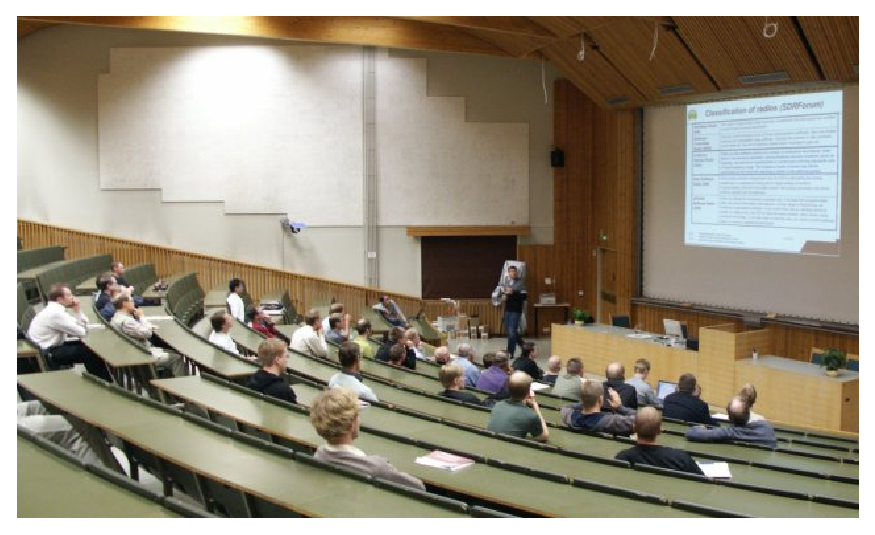
\includegraphics[height=8cm]{kuva2}
\end{center}
\caption{Kuvateksti, jossa on liitteen numerointi}
\label{liitekuva}
\end{figure}
%%
Liitteiden taulukoiden numerointi on kuvien ja kaavojen kaltainen:
\begin{table}[htb]
\caption{Taulukon kuvateksti.}
\label{liitetaulukko}
\begin{center}
\fbox{
\begin{tabular}{lp{0.5\linewidth}}
9.00--9.55  & K\"aytett\"avyystestauksen tiedotustilaisuus (osanottajat
ovat saaneet s\"ahk\"opostitse valmistautumisteht\"av\"at, joten tiedotustilaisuus
voidaan pit\"a\"a lyhyen\"a).\\
9.55--10.00 & Testausalueelle siirtyminen
\end{tabular}}
\end{center}
\end{table}
Kaavojen numerointi muodostaa liitteiss\"a oman kokonaisuutensa:
\begin{eqnarray}
T_{ik} &=& -p g_{ik} + w u_i u_k + \tau_{ik},  \label{liitekaava3} \\
n_i    &=& n u_i + v_i.                      \label{liitekaava4}
\end{eqnarray}

\end{document}
